\documentclass{article}%
\usepackage[T1]{fontenc}%
\usepackage[utf8]{inputenc}%
\usepackage{lmodern}%
\usepackage{textcomp}%
\usepackage{lastpage}%
\usepackage{authblk}%
\usepackage{graphicx}%
%
\title{Mannheimia haemolytica Leukotoxin Activates a Nonreceptor Tyrosine Kinase Signaling Cascade in Bovine Leukocytes, Which Induces Biological Effects}%
\author{Kevin Campbell}%
\affil{Department of Medicine, Addenbrooke's Hospital, University of Cambridge, Cambridge, United Kingdom}%
\date{01{-}01{-}2012}%
%
\begin{document}%
\normalsize%
\maketitle%
\section{Abstract}%
\label{sec:Abstract}%
Even if he's had his medicine for colorectal cancer several times before, it appears that Lon Silver has detected it at different times.\newline%
Silver, a Dana{-}Farber Cancer Institute gastroenterologist who has been doing his rounds at the cancer center, reported Sunday that he has found that one particular antibody that differs between the prostate and colorectal cancer patients.\newline%
It's true, he said.\newline%
The difference may not be as big a deal as one would think. It could be that not all patients who develop colorectal cancer develop the same type of antibodies to prostate cancer, he explained.\newline%
As it happens, the men with the different kinds of antibody did not develop prostate cancer as easily. And in this case, the antibody that was focused on colorectal cancer was not even tested for prostate cancer, Silver said. The only way doctors can tell if a patient who has an earlier stage prostate cancer will eventually develop colorectal cancer is to intervene sooner, by surgery or chemotherapy, he explained.\newline%
Doctors don't just test for prostate cancer in some patients.\newline%
They test for other diseases, too, including cerebrovascular disease and heart disease. Patients with bad heart valves and bad blood vessels, for example, can get tests for heart disease just as easily.\newline%
But while some patients develop heart disease early and gradually, those who have a poor fitness level and die younger, can be cured with surgery, Silver said.\newline%
Also, some people develop colorectal cancer early on and, as a result, can have or start the disease as a young adult. In that case, doctors are able to screen more patients and possibly spot the early disease, he said.\newline%
So it's not yet time to panic.\newline%
"But the good news is that we do detect it and treat it now," Silver said.\newline%
And the second{-}most important thing, Silver said, is to find the right individual.

%
\subsection{Image Analysis}%
\label{subsec:ImageAnalysis}%


\begin{figure}[h!]%
\centering%
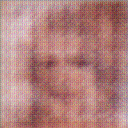
\includegraphics[width=150px]{500_fake_images/samples_5_466.png}%
\caption{A Close Up Of A Black And White Picture Of A Black And White Cat}%
\end{figure}

%
\end{document}